\documentclass[11pt]{article}
\usepackage{../EllioStyle}
\usepackage{graphicx}

\title{Homework 5}
\author{Elliott Pryor \\
Collaborated with: Nathan Stouffer}
\date{25 March 2021}

\rhead{Homework 5}
\lhead{Elliott Pryor}

\graphicspath{{./}{images/}}




\makeatletter
\def\mathcolor#1#{\@mathcolor{#1}}
\def\@mathcolor#1#2#3{%
  \protect\leavevmode
  \begingroup
    \color#1{#2}#3%
  \endgroup
}
\makeatother


\algdef{SE}[DOWHILE]{Do}{doWhile}{\algorithmicdo}[1]{\algorithmicwhile\ #1}

\begin{document}

\maketitle


\problem{1}

In Homework 1, we considered a plane-sweep algorithm for determining whether
there is any intersection among a collection of $n$ circles in the plane. Here
we consider a variant of this problem. The input consists of a collection of $n$
closed circular disks, all having the same radius. (Via scaling, we may assume
that they are all unit disks.) Let $C = \{c_1, \ldots , c_n\}$ denote the center
points of these disks, and let $\{D_1, \ldots, D_n\}$ denote the actual disks.
Thus, $D_i$ consists of the points that lie within unit distance of $c_i$. Let
$U = D_1 \cup \ldots \cup D_n$ denote the union of these disks. The boundary of
$U$ may generally consist of multiple parts, each of which consists of a cycle
of circular arcs connected by vertices. (In Fig. 4 the boundary consists of
three cycles. The vertices are shown as white dots).

\begin{figure}[h]
    \centering
    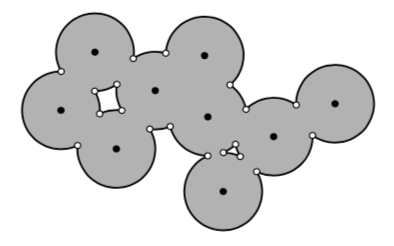
\includegraphics[width=0.4\textwidth]{union-of-disks}
    \caption{Problem 4: Union of disks}
\end{figure}

\begin{enumerate}

    \item Present an algorithm that reports all the vertices on the boundary of
        $U$. (Note that circle intersection points in the interior of the union
        are explicitly excluded.) Your algorithm should run in time $O(n log
        n)$.  The order in which the vertices are output is arbitrary. (Hint:
        Don't try to modify the algorithm from Homework 2. A different approach
        is needed.... think giraffes)

    \item Prove that the number of vertices reported by your algorithm is
        $O(n)$.

\end{enumerate}

\hrule





\begin{algorithm}[H]
    \caption{Verticies of Disks}
    \label{alg:neighbors}
    \begin{algorithmic}[1]
    \Function{disks}{$C$}
        \State Voronoi = Voronoi Diagram($C$)
        \State $P \gets []$
        \For{$c \in C$}
            \For{edge in Voronoi around cite $c$}
                \State if circle of radius 1 intersects edge, add it to $P$
            \EndFor
        \EndFor
        \State \textbf{return: } $P$
    \EndFunction
    \end{algorithmic}
\end{algorithm}


We assume that there are no isolated circles (or if there are we do not need to report them).
This could also be checked easily and still computed in $O(n \log n)$ if needed.
We also assume that the disks are closed, so if there is an intersection of 3 circles
at one point (vertex in voronoi) this does not count as hole in the union of disks.

\textbf{Runtime: }
This runs in $O(n \log n)$. We can compute the voronoi diagram (line 2)
using Fortune's algorithm on $O(n \log n)$. 
Then there are $n$ centers we look at in the first for loop.
From Euler's formula, we know that $|E| = O(n)$, that means around each center (face)
there are $O(1)$ edges. Thus the inner loop is $O(1)$ time (we can compute intersection in $O(1)$ time).

\textbf{Correctness: }
The correctness hinges on the following theorem,
a vertex is on the boundary iff the circle of radius 1 intersects the voronoi
edge belonging to the face in which the circle's center is the site. 

\begin{proof}
    We prove the reverse direction. 

    We first establish that if there is an intersection of circle and a voronoi edge,
    then there is an intersection of circles at that point. From the circle property,
    a point on a voronoi edge has a circle of some radius that touches 2 sites.
    Since there was an intersection of the edge with the circle, we know that the point is 
    exactly distance $R$ ($R=1$) from the first site, thus there must be another site at distance $R$
    from that point. Since all disks are of radius $R$, there is an intersection of the 2 disks at that point.

    We then show that this must be on the boundary (exterior). If the intersection occurs on a voronoi
    edge not belonging to this center, then the point on the voronoi edge is closer to 2 other sites,
    thus it is within them. So we only need to consider the voronoi edges belonging to the centers.

    Suppose that this intersection is in the interior. Then there must be another circle such that 
    the distance to the point is less than $R$ (1 in our case). 
    Then this point is not equidistant between our site and this other site. Thus it cannot be along the
    voronoi edge belonging to this site. A contradiction. Thus it must be exterior.
\end{proof}

We don't need to prove the forward direction for the correctness of the algorithm. 
So thus our algorithm does find the exterior intersections as required. 




\problem{2}

Suppose we are given a subdivision of the plane into $n$ convex regions. We
suspect that this subdivision is a Voronoi diagram, but we do not know the
sites. Develop an algorithm that finds a set of $n$ point sites whose Voronoi
diagram is exactly the given subdivision, if such a set exists.
\hrule




\end{document}